\section{Τριφασικός Ανορθωτής}

Προσομοιώθηκε το κύκλωμα του τριφασικού μετασχηματιστή όπως αυτό φαίνεται στο fig:\ref{img:3_phase}.
\begin{figure}[h]
	\centering
	\includegraphics[width = 0.5\textwidth]{Images/3_phase.png}
	\caption{Κύκλωμα Τριφασικού Ανορθωτή}
	\label{img:3_phase}
\end{figure}

\noindent
Σε αντίθεση με τον μονοφασικό μετασχηματιστή, χρησιμοποιούνται 6 Thyristor όμως και πάλι σε κάθε χρονική στιγμή άγουν μόνο δύο Thyristor, ένα από την πάνω πλευρά και ένα από την κάτω. Και σε αυτή την περίπτωση το φορτίο είναι RL.

\noindent\\
Ομοίως με τον μονοφασικό ανορθωτή, υπολογίζονται οι παράμετροι Α, Β, C, D και στην συνέχεια δημιουργείται το συνεχές και το διακριτό σύστημα μέσω των συναρτήσεων ss και c2d αντίστοιχα. Για κάθε σημείο του διακριτού σήματος, υπολογίζεται η γωνία ω η οποία και πάλι περιορίζεται σε τιμές μεταξύ [0 2π].

\noindent\\
ΝΑ ΤΑ ΠΕΙΣ ΣΤΟ ΠΡΏΤΟ ΜΈΡΟΣ
Σε αντίθεση με τον μονοφασικό ανορθωτή, η εναλλαγή μεταξύ των τάσεων γίνεται κάθε $60^o$ και όπως προαναφέρθηκε στην υποενότητα .  ???????????

\subsection{Γωνία έναυσης 0 μοίρες για L=0.04Η και L=0.08Η}

\subsubsection{Τάση εξόδου}

\begin{figure}[h]
	\centering
	\begin{subfigure}{.5\textwidth}
		\centering
		\includegraphics[width = 0.9\linewidth]{Images/3_Vout_0_04}
		\caption{a = 0, L = 0.04}
		\label{fig:3_vout_0_04}
	\end{subfigure}%
	\begin{subfigure}{.5\textwidth}
		\centering
		\includegraphics[width = 0.9\linewidth]{Images/3_Vout_0_08}
		\caption{a = 0, L = 0.04}
		\label{fig:3_vout_0_08}
	\end{subfigure}
	\caption{$V_{out} $ vs $V_{in}$ (a=0 L=0.04/0.08)}
	\label{figs:3_vout_0}
\end{figure}

\noindent
Έχοντας θέσει την γωνία έναυσης ίση με 0, τα thyristor πρακτικά λειτουργούν ως μην ελεγχόμενες δίοδοι και ως αποτέλεσμα η τάση εξόδου είναι θετική και πιο συγκεκριμένα να ακολουθεί πάντα την υψηλότερη τάση. Αυτό συμβαίνει καθώς ως απλές δίοδοι άγουν μόνο όταν είναι ορθά πολωμένες και όπως προαναφέρθηκε στην υποενότητα \ref {} άγουν μόνο οι δίοδοι που είναι πιο ορθά πολωμένες. Τέλος, όπως ήταν αναμενόμενο, η τάση εξόδου δεν επηρεάζεται από την μεταβολή της αυτεπαγωγής L όπως προαναφέρθηκε στην υποενότητα \ref{}


\subsubsection{Ρεύμα εξόδου}

\begin{figure}[h]
	\centering
	\begin{subfigure}{.5\textwidth}
		\centering
		\includegraphics[width =1\textwidth]{Images/3_Iout_0_04}
		\caption{a = 0, L = 0.04}
		\label{fig:3_iout_0_04}
	\end{subfigure}%
	\begin{subfigure}{.5\textwidth}
		\centering
		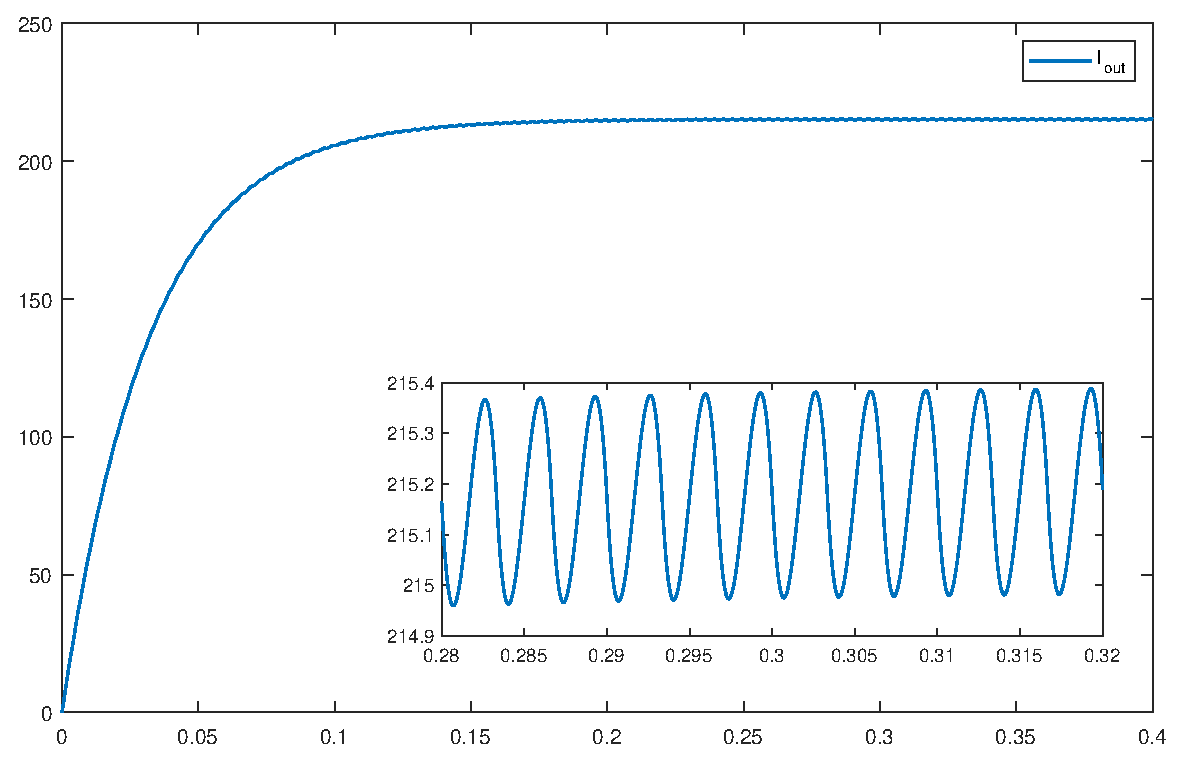
\includegraphics[width = 1\textwidth]{Images/3_Iout_0_08}
		\caption{a = 0, L = 0.04}
		\label{fig:3_iout_0_08}
	\end{subfigure}
	\caption{$I_{out} $ (a=0 L=0.04/0.08)}
	\label{figs:3_iout_0}
\end{figure}


Όπως προαναφέρθηκε, εφόσον τα thyristor λειτουργούν ως απλές δίοδοι, το ρεύμα όπως ήταν αναμενόμενο δεν παρουσιάζουν ιδιαίτερες διακυμάνσεις. Πιο συγκεκριμένα, για L = 0.04 H η διακύμανση του ρεύματος, εφόσον αυτό έχει σταθεροποιηθεί είναι ίση με 0.8Α ενώ για L = 0.08 η διακύμανση είναι ίση με (ΒΆΛΕ DATA TIPS ΚΑΙ ΠΕΣ ΠΌΣΟ ΕΊΝΑΙ), δηλαδή παρατηρείται μία μείωση της τάξης των ??\%.

Ακόμα, παρατηρείται πως η αύξηση της αυτεπαγωγής επιδρά με δύό τρόπους στο κύκλωμα. Πρώτον μειώνονται οι διακυμάνσεις του ρεύματος, δηλαδή το ρεύμα εξόδου προσομοιάζει καλύτερα το DC ρεύμα και δεύτερον αυξάνεται ο χρόνος σταθεροποίησης, δηλαδή απαιτείται μεγαλύτερο χρονικό διάστημα έως ότου φτάσει στην τελική του τιμή. Όσον αφορά την μείωση των διακυμάνσεων, η αύξηση της αυτεπαγωγής συνεπάγεται ΠΕΣ ΟΤΙ ΔΕΝ ΑΝΤΙΔΡΆ ΤΌΣΟ ΓΡΉΓΟΡΑ. Όσον αφορά τον χρόνο σταθεροποίηση, προκύπτει μέσω της σχέσης τ = $\frac{L}{R}$ και άρα είναι ανάλογη της αυτεπαγωγής.

Τέλος, το ρεύμα δεν μηδενίζεται οπότε η λειτουργία είναι συνεχής.


\subsubsection{Ρεύμα Thyristor}
\begin{figure}[h]
	\centering
	\begin{subfigure}{.5\textwidth}
		\centering
		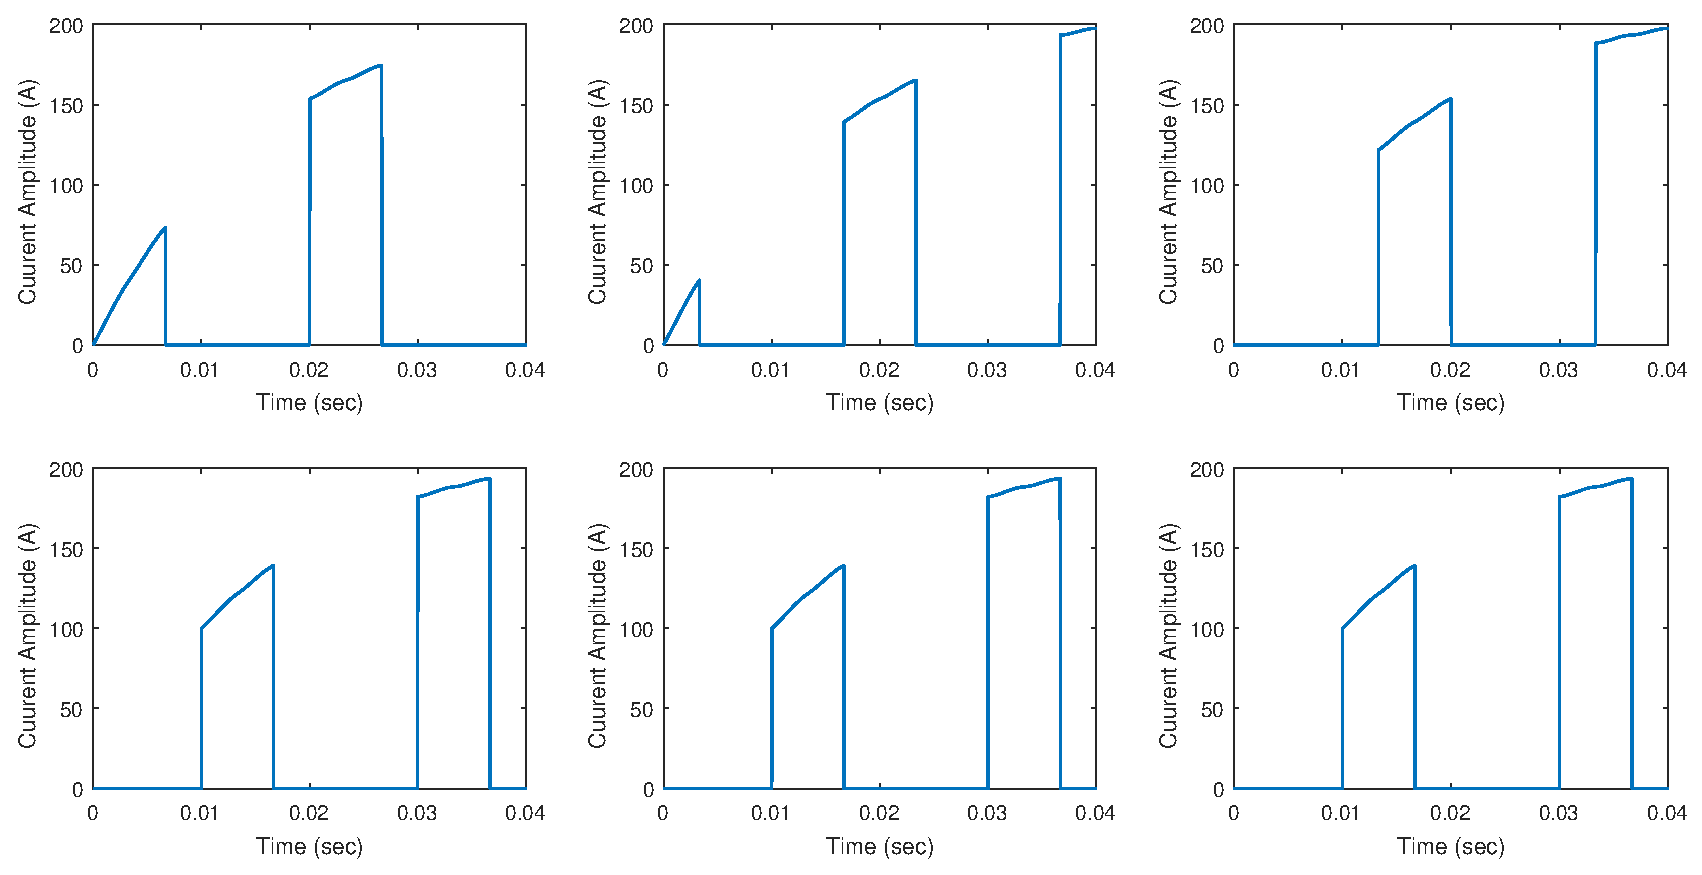
\includegraphics[width =0.9\textwidth]{Images/3_ThI_0_04}
		\caption{a = 0, L = 0.04}
		\label{fig:3_ThI_0_04}
	\end{subfigure}%
	\begin{subfigure}{.5\textwidth}
		\centering
		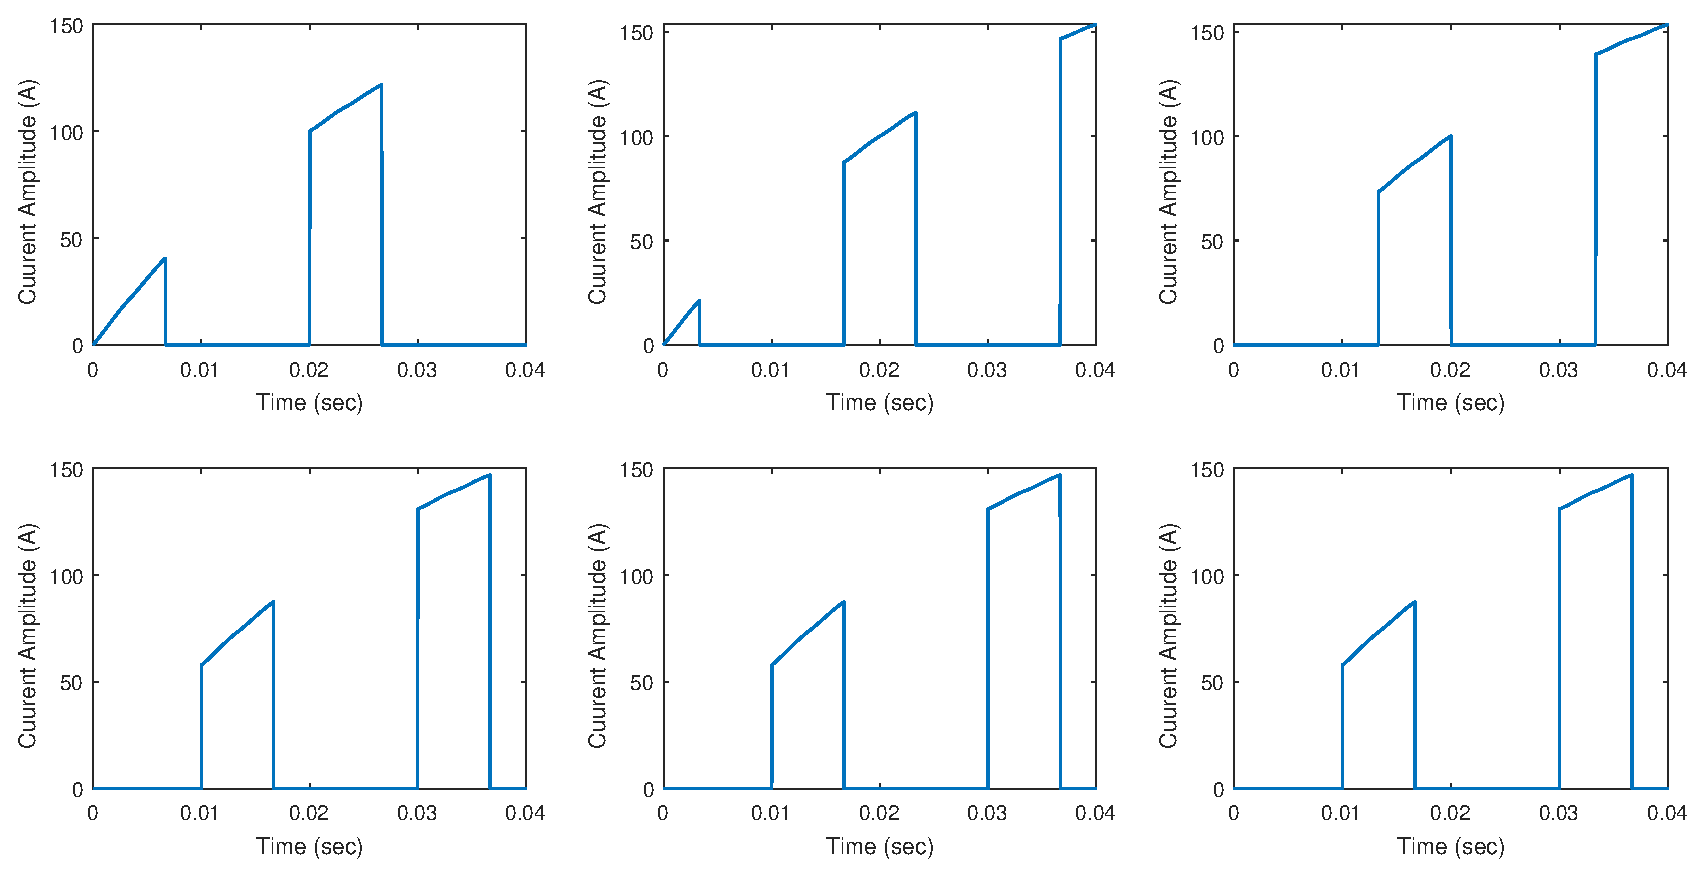
\includegraphics[width = 0.9\textwidth]{Images/3_ThI_0_08}
		\caption{a = 0, L = 0.08}
		\label{fig:3_ThI_0_08}
	\end{subfigure}
	\caption{Thyristor Currents (a=0 L=0.04/0.08)}
	\label{figs:3_ThI_0}
\end{figure}

Το figures \ref{figs:3_ThI_0} αναπαριστούν το ρεύμα σε κάθε Thyristor για χρόνο 2 περιόδων. Το ρεύμα της διόδου είναι ίσο με το ρεύμα εξόδου όταν αυτή άγει εφόσον θεωρούνται ιδανικές. Οι δίοδοι άγουν σύμφωνα με τον πίνακα της υποενότητας.....
